\subsection{تخمین پارامتر کانال‌های رول-پیچ-یاو}
برای اصلاح پارامترها رول-پیچ چندین آزمایش انجام شد و با استفاده از داده‌های ثبت شده از وضعیت استند در کانال رول-پپچ-یاو و جعبه‌ابزار
\lr{Parameter Estimator}
پارامترهای کانال رول-پیچ-یاو اصلاح شدند.
برای آزمایش تمامی موتورها با دور مختلف شروع به حرکت کردند و از خروجی سنسور داده برداری شد. سپس، مدل و  داده‌های ثبت شده سنسور (وضعیت استند در کانال رول-پیج-یاو) به جعبه‌ابزار
\lr{Parameter Estimator}
داده شد. وضعیت کانال رول-پیچ-یاو استند در شبیه‌سازی و واقعیت بعد از اصلاح پارامترهای کانال‌ رول-پیچ-یاو بعد در شکل‌های
(\ref{ roll_pitch_yaw_ps1}, \ref{ roll_pitch_yaw_ps2}, \ref{ roll_pitch_yaw_ps3}, \ref{ roll_pitch_yaw_ps4}, \ref{ roll_pitch_yaw_ps5}, \ref{ roll_pitch_yaw_ps6}, \ref{ roll_pitch_yaw_ps7}, \ref{ roll_pitch_yaw_ps8}, \ref{ roll_pitch_yaw_ps9})
آورده شده است.

\begin{figure}[H]
	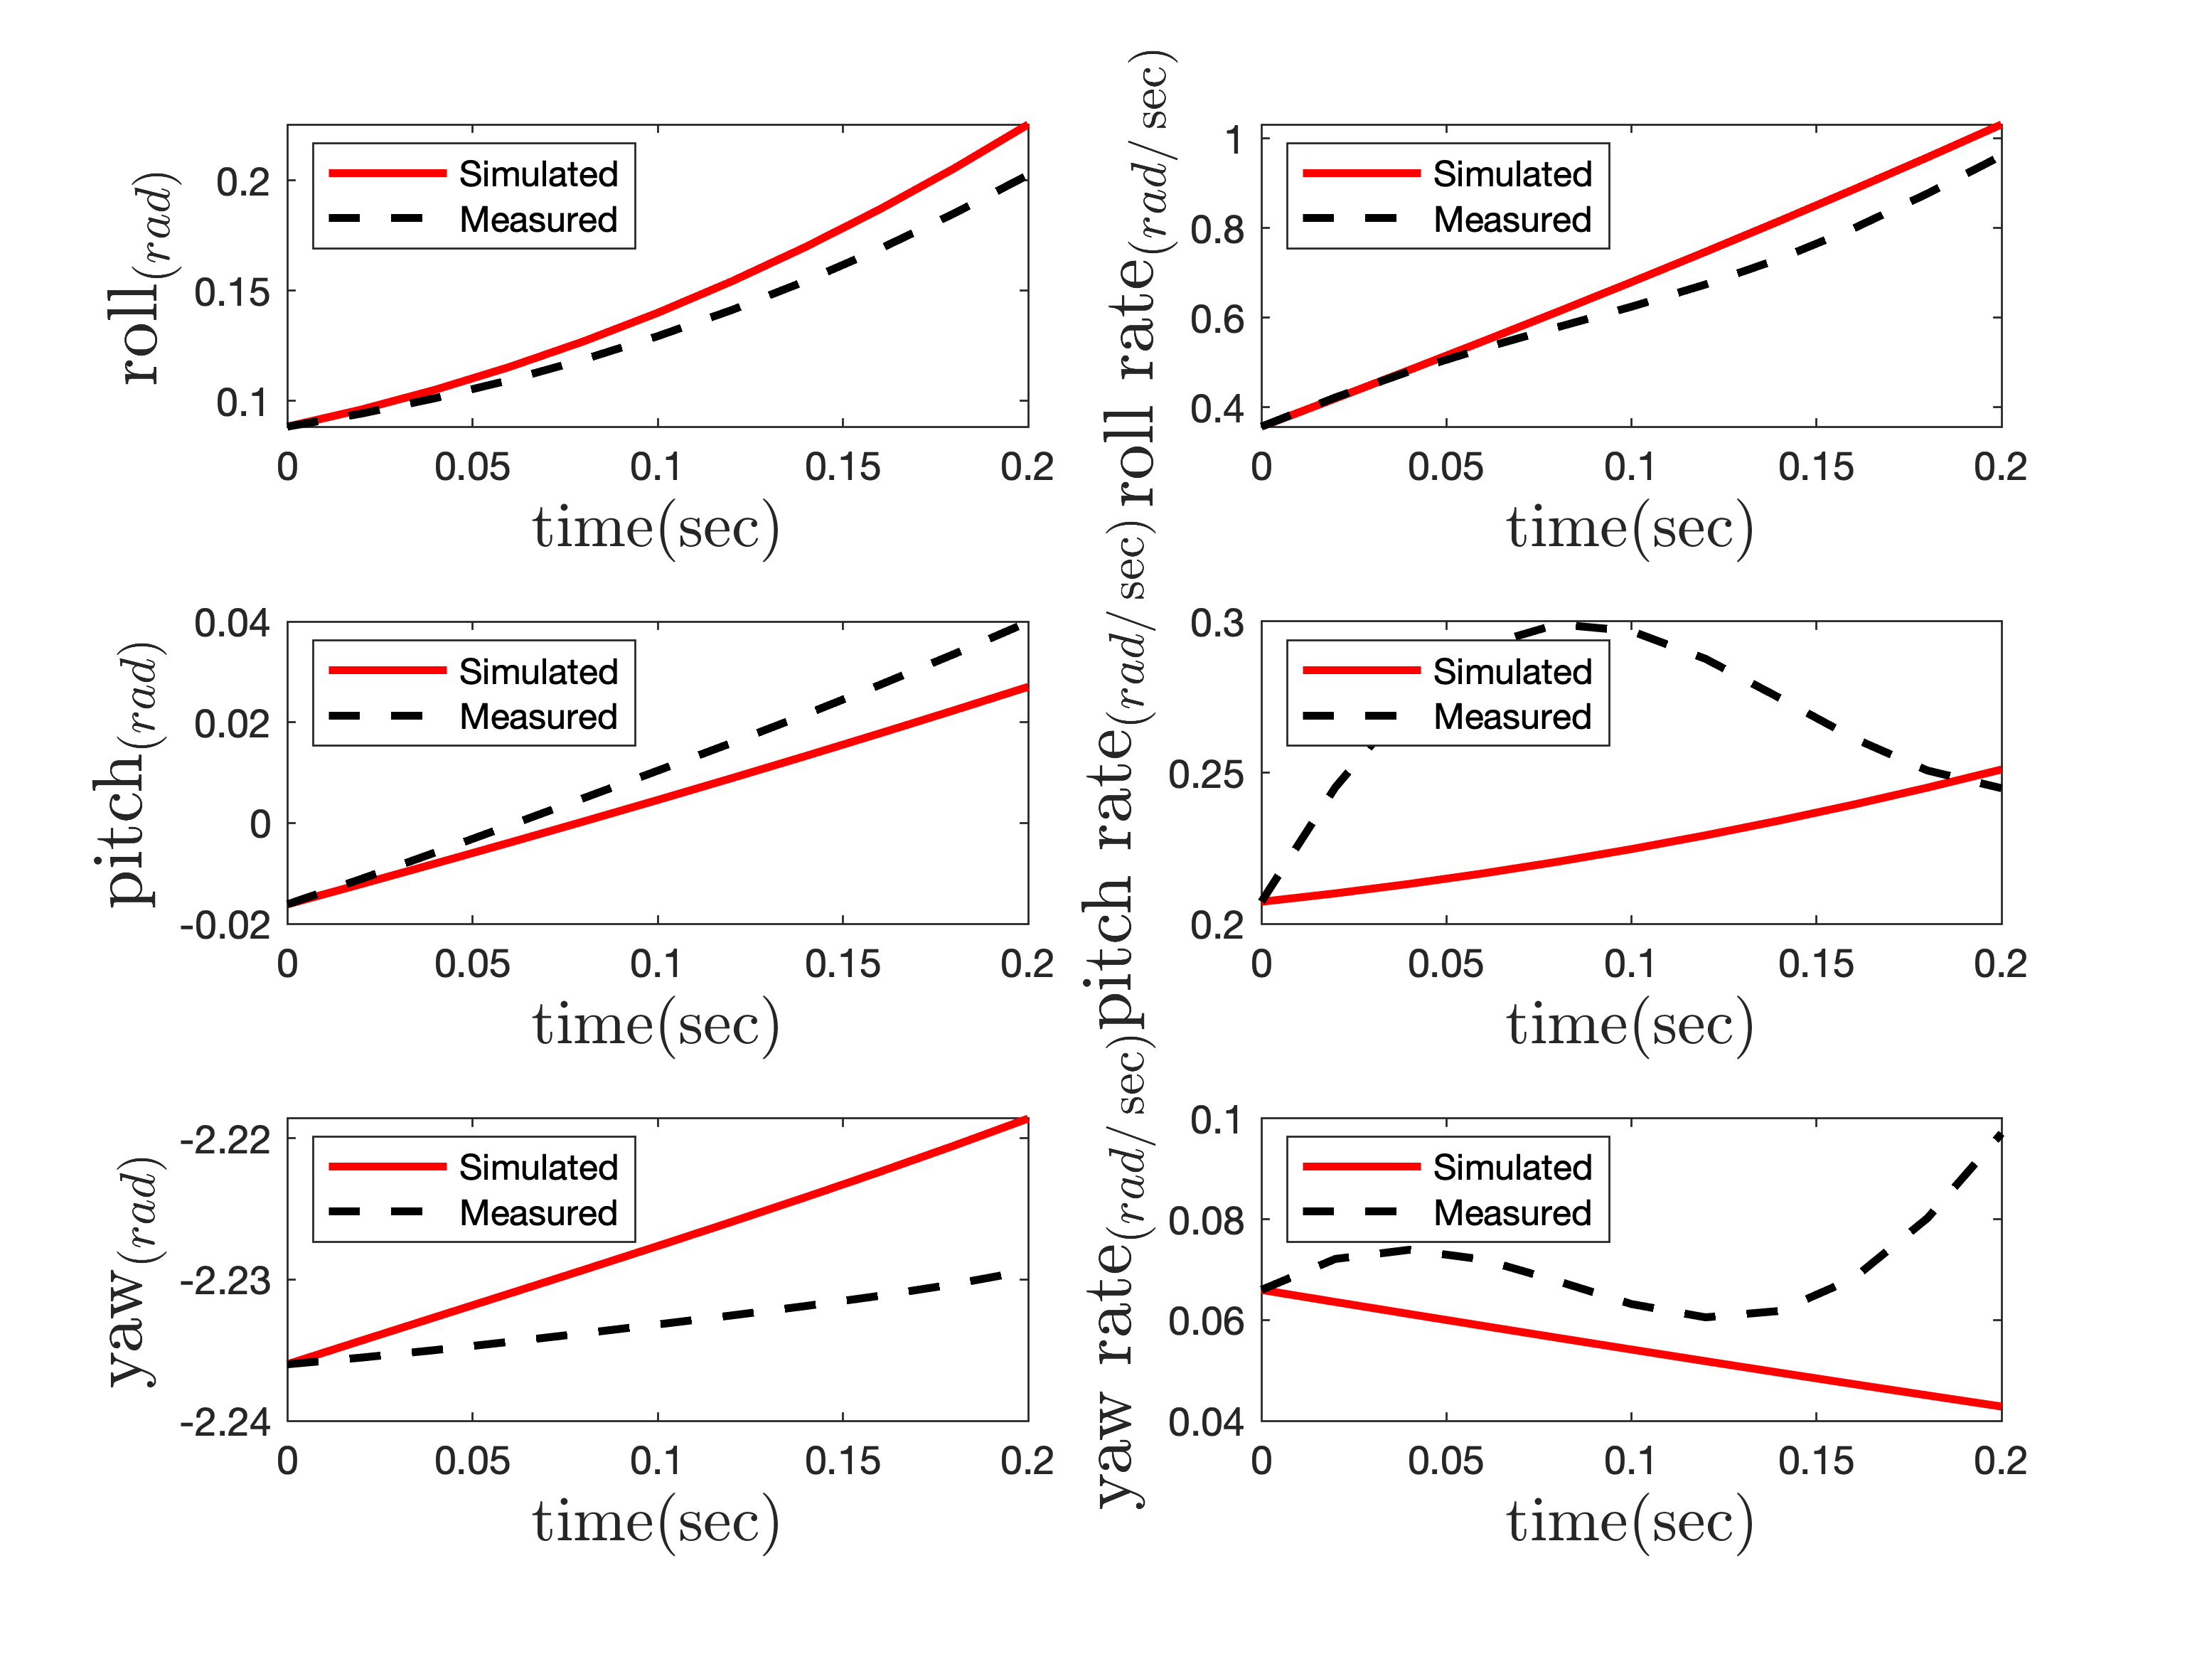
\includegraphics[width=12cm]{../../Figures/RCP/roll_pitch_yaw_parameter_estimation/RCP_roll_pitch_yaw_S1.png}
	\centering
	\caption{مقايسه وضعیت استند در  آزمايش اول و شبیه‌سازی، پس از تخمین پارامترهای کانال رول-پیچ-یاو}
	\label{ roll_pitch_yaw_ps1}
\end{figure}
\begin{figure}[H]
	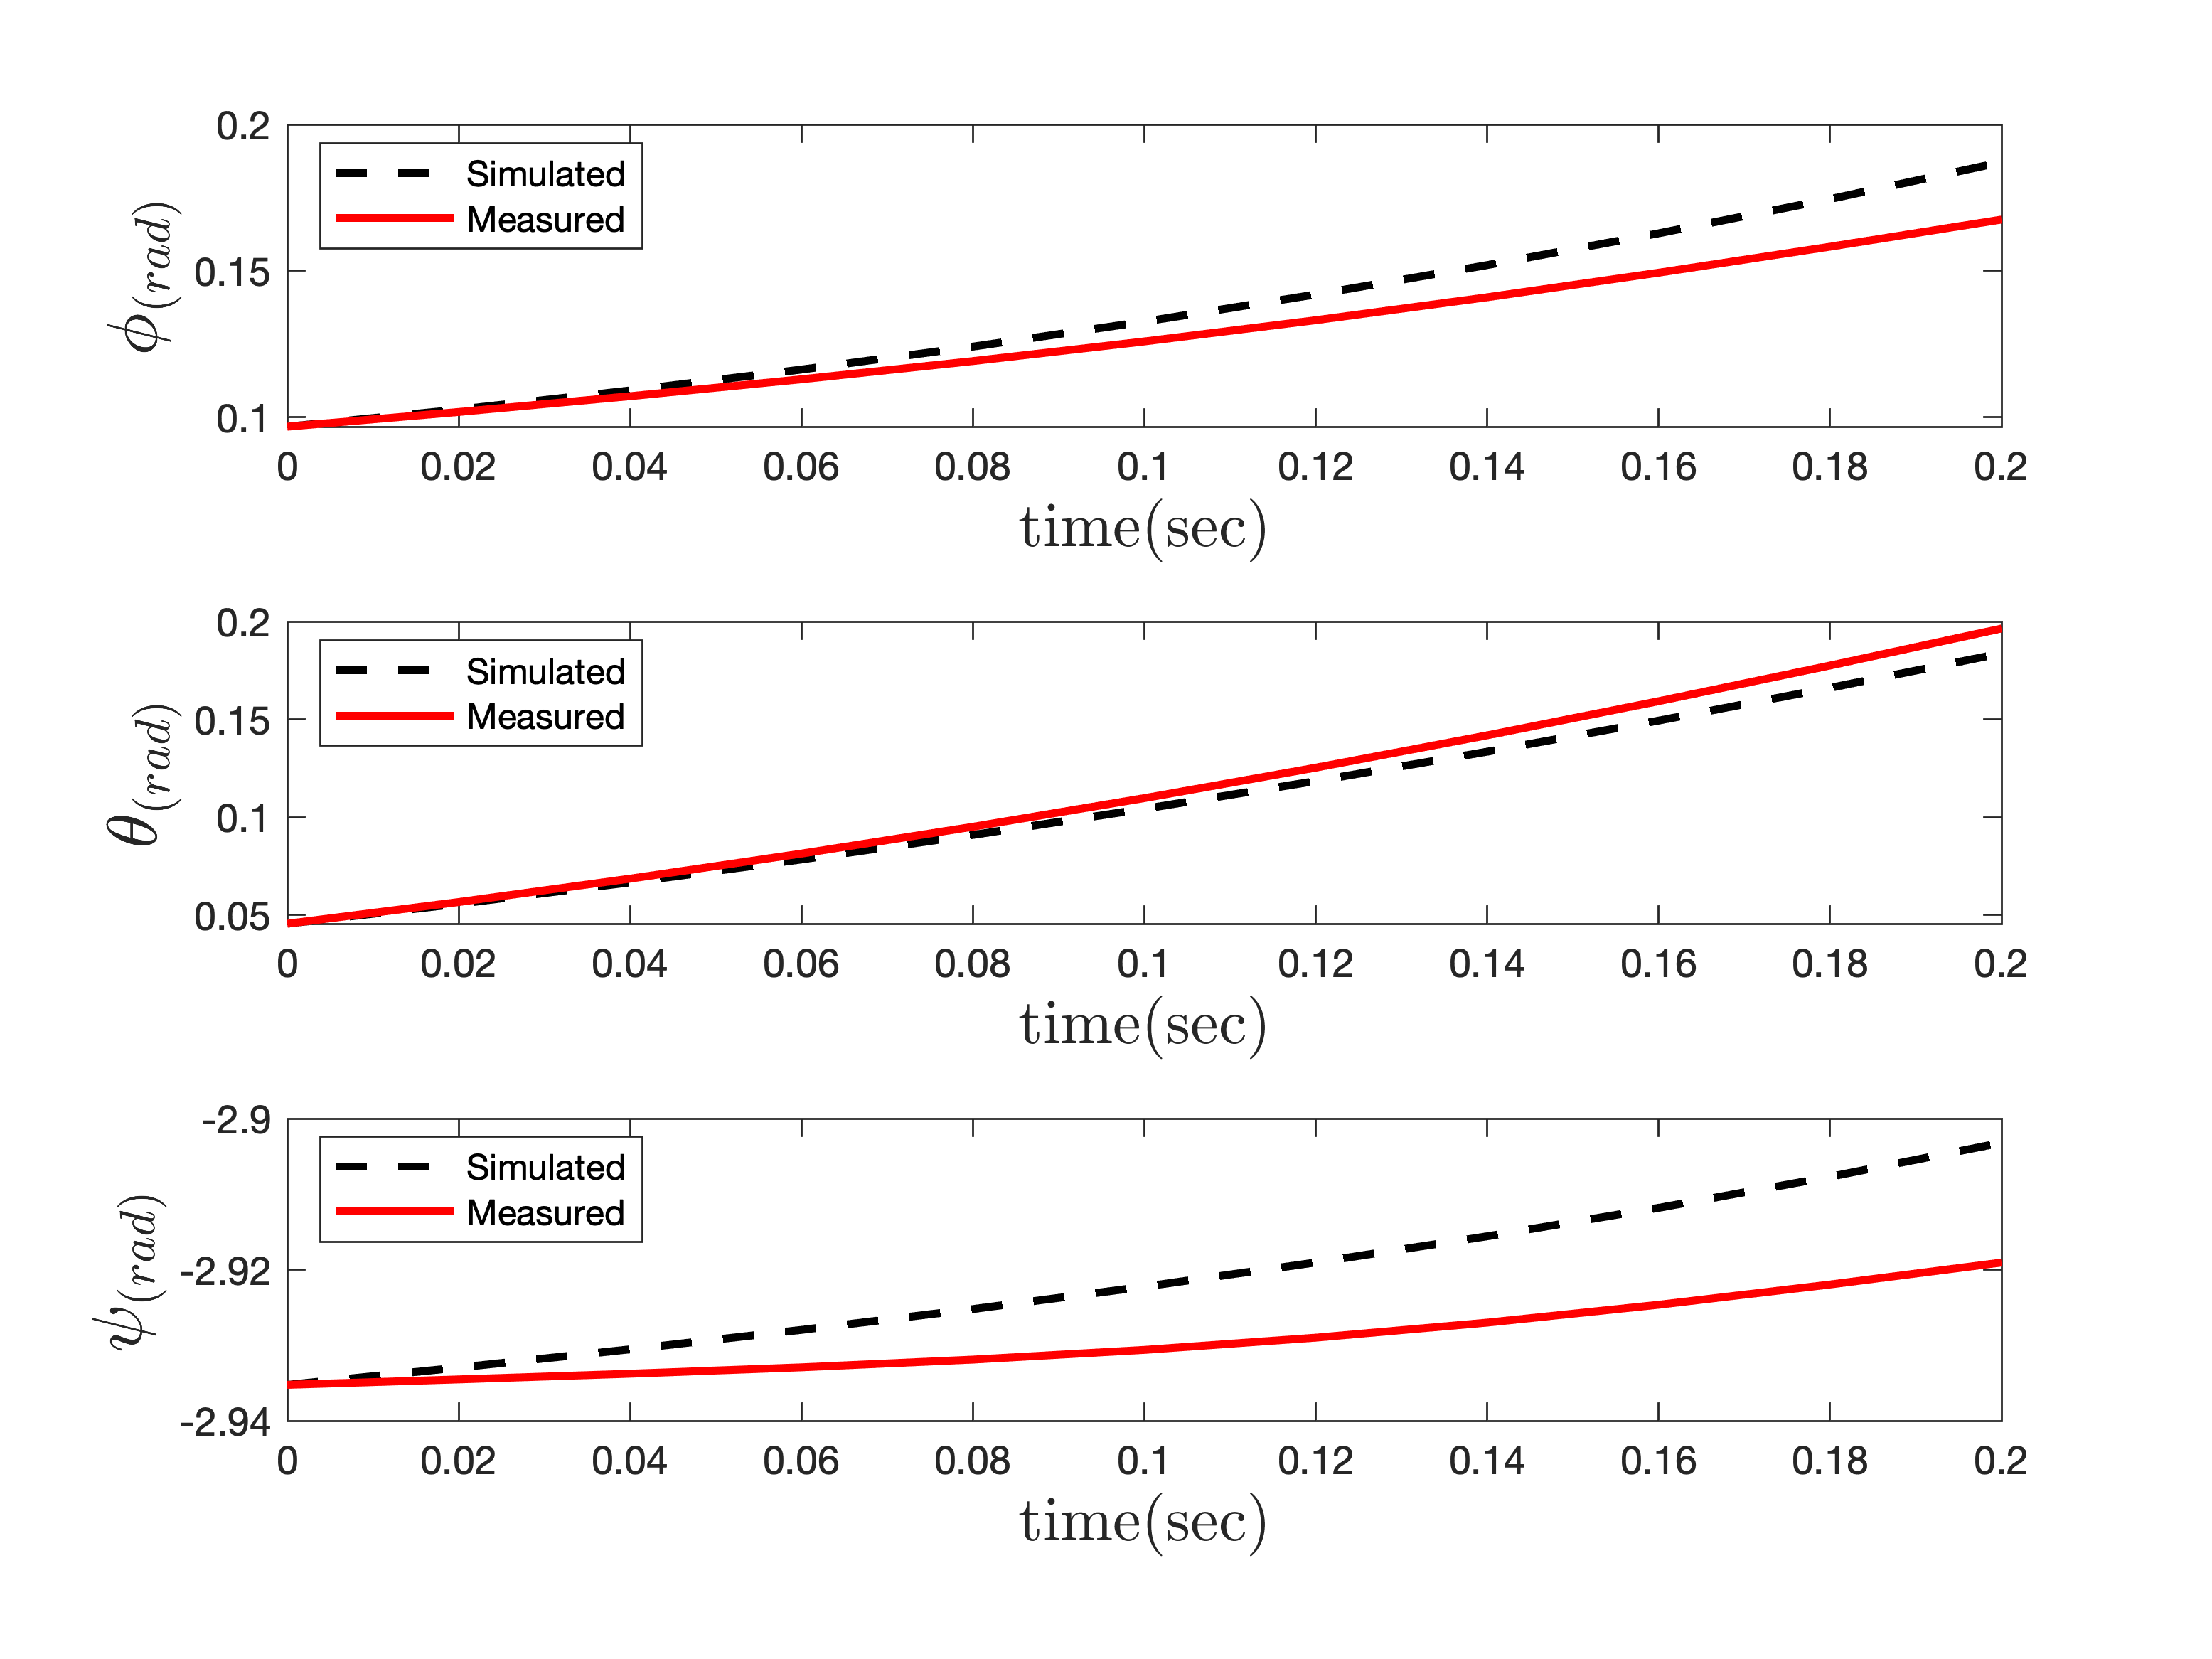
\includegraphics[width=12cm]{../../Figures/RCP/roll_pitch_yaw_parameter_estimation/RCP_roll_pitch_yaw_S2.png}
	\centering
	\caption{مقايسه وضعیت استند در  آزمايش دوم و شبیه‌سازی، پس از تخمین پارامترهای کانال رول-پیچ-یاو}
	\label{ roll_pitch_yaw_ps2}
\end{figure}
\begin{figure}[H]
	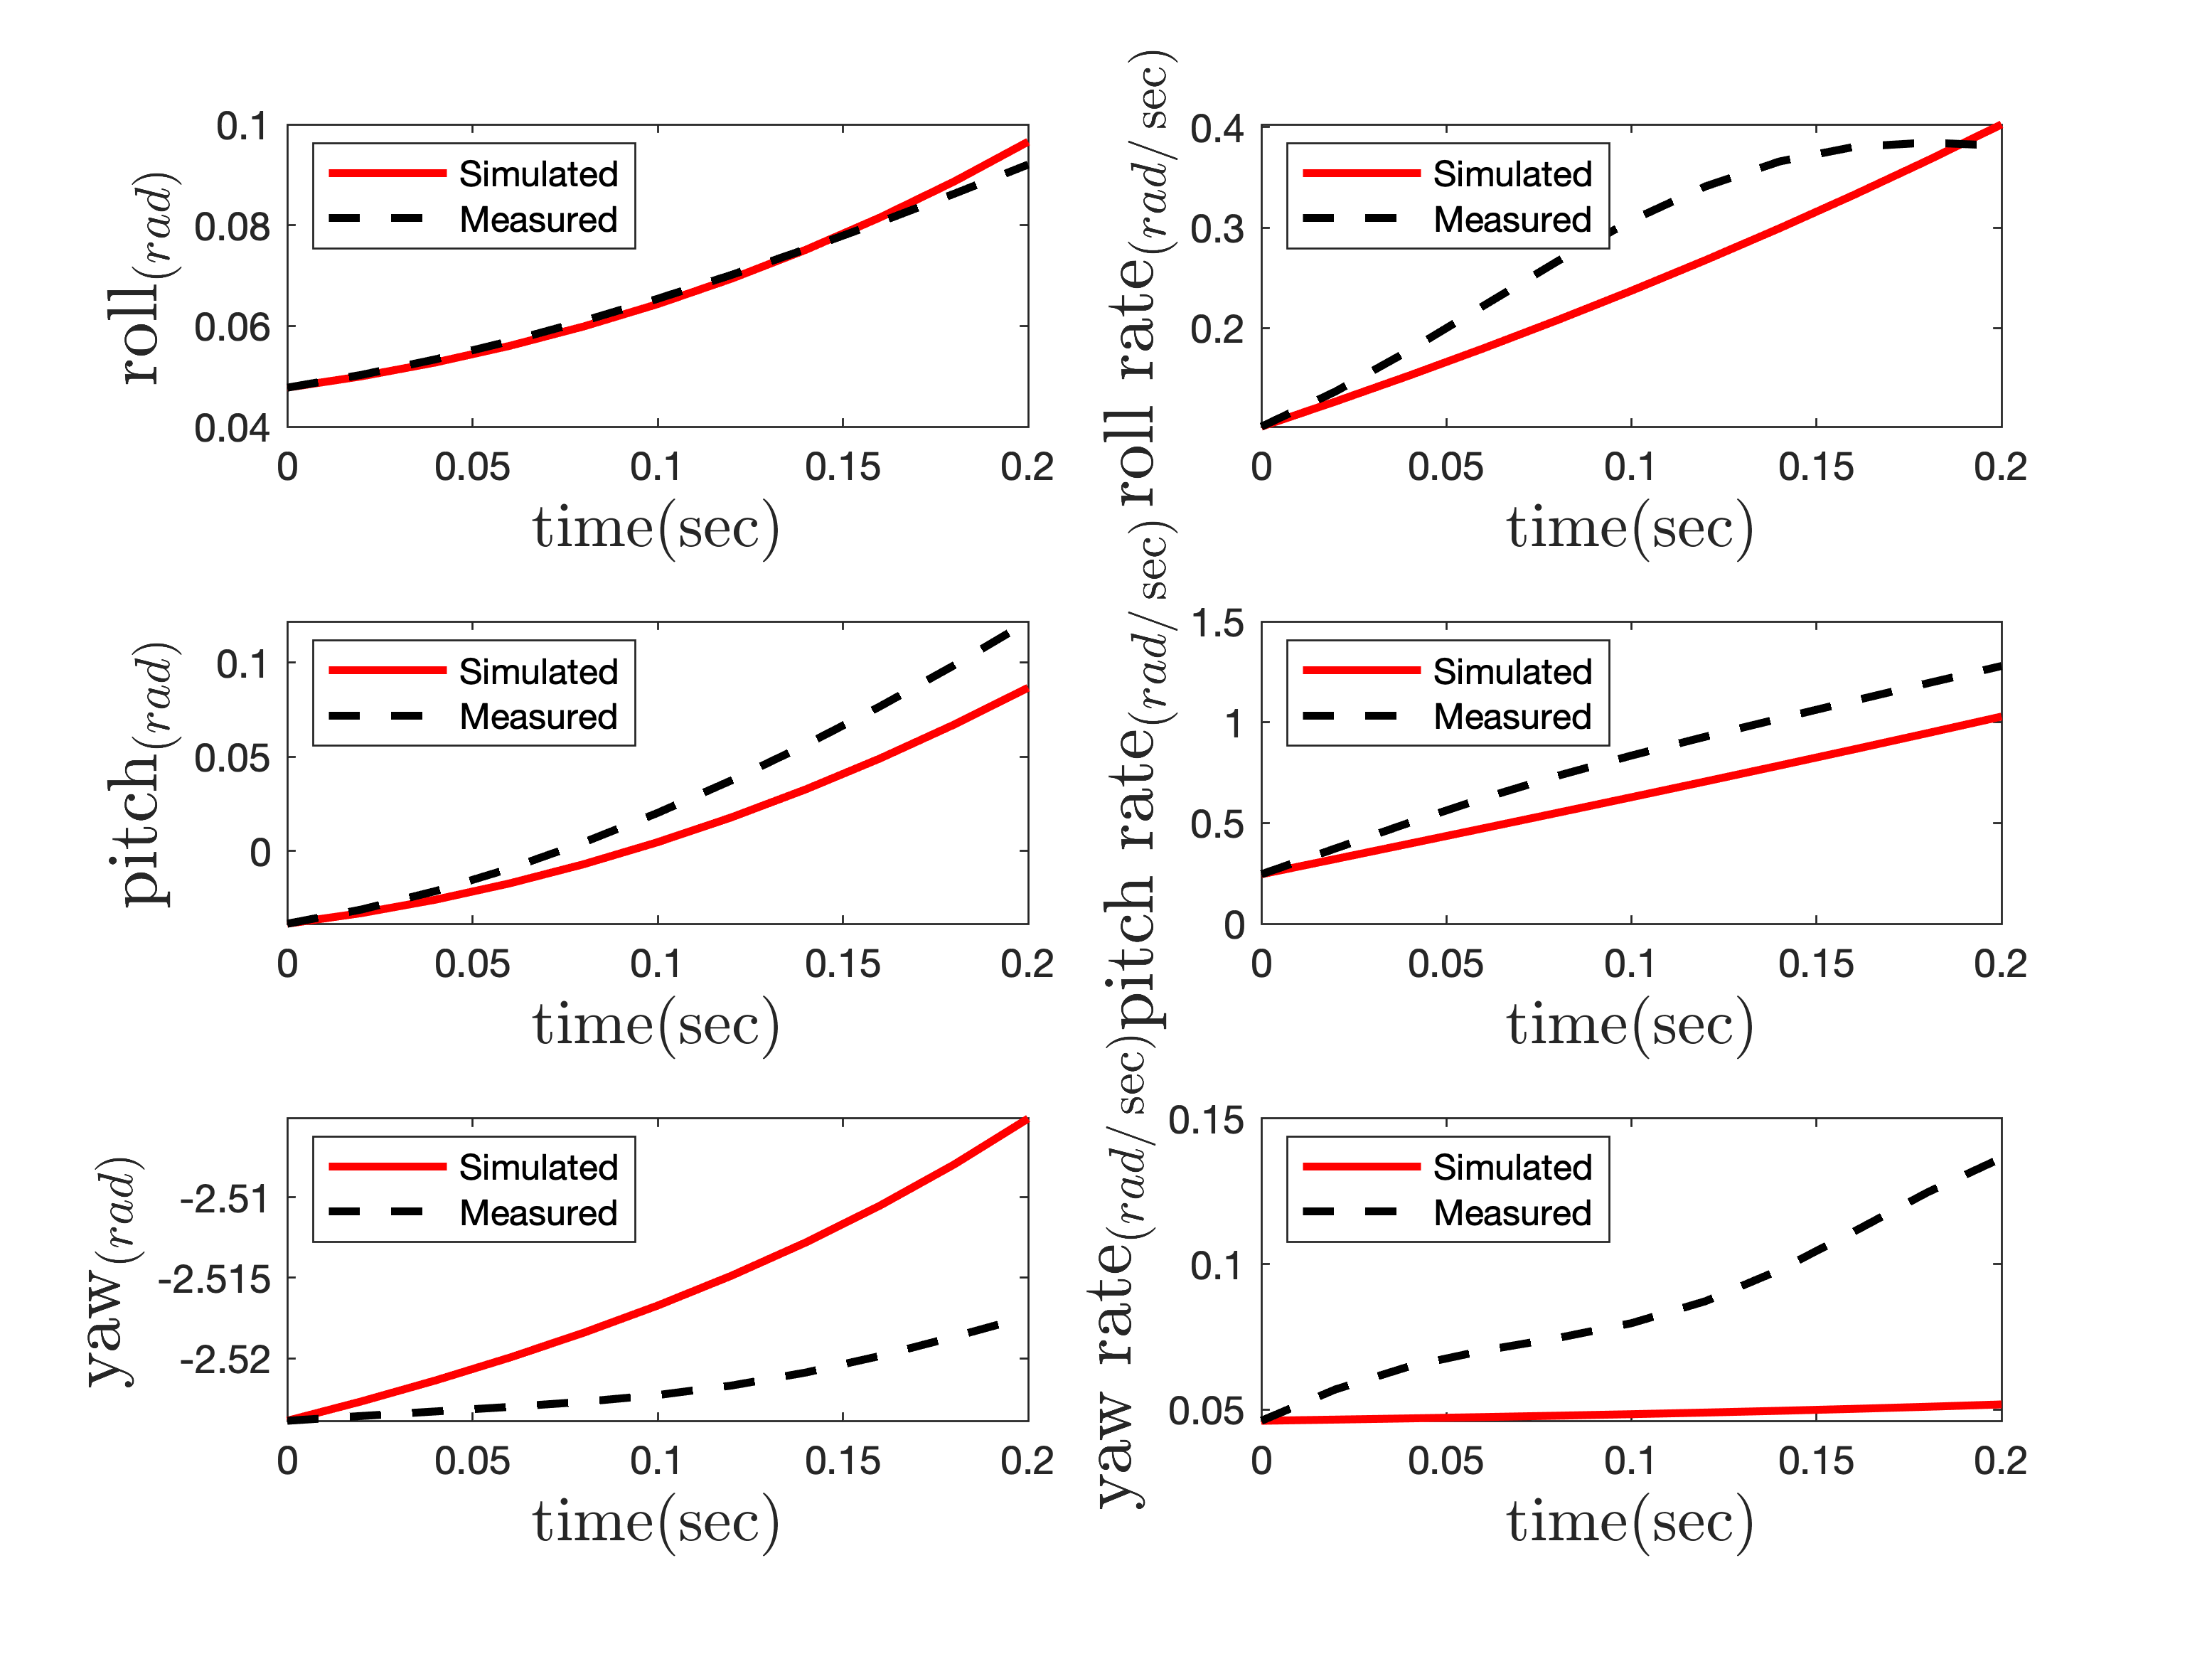
\includegraphics[width=12cm]{../../Figures/RCP/roll_pitch_yaw_parameter_estimation/RCP_roll_pitch_yaw_S3.png}
	\centering
	\caption{مقايسه وضعیت استند در  آزمايش سوم و شبیه‌سازی، پس از تخمین پارامترهای کانال رول-پیچ-یاو}
	\label{ roll_pitch_yaw_ps3}
\end{figure}
\begin{figure}[H]
	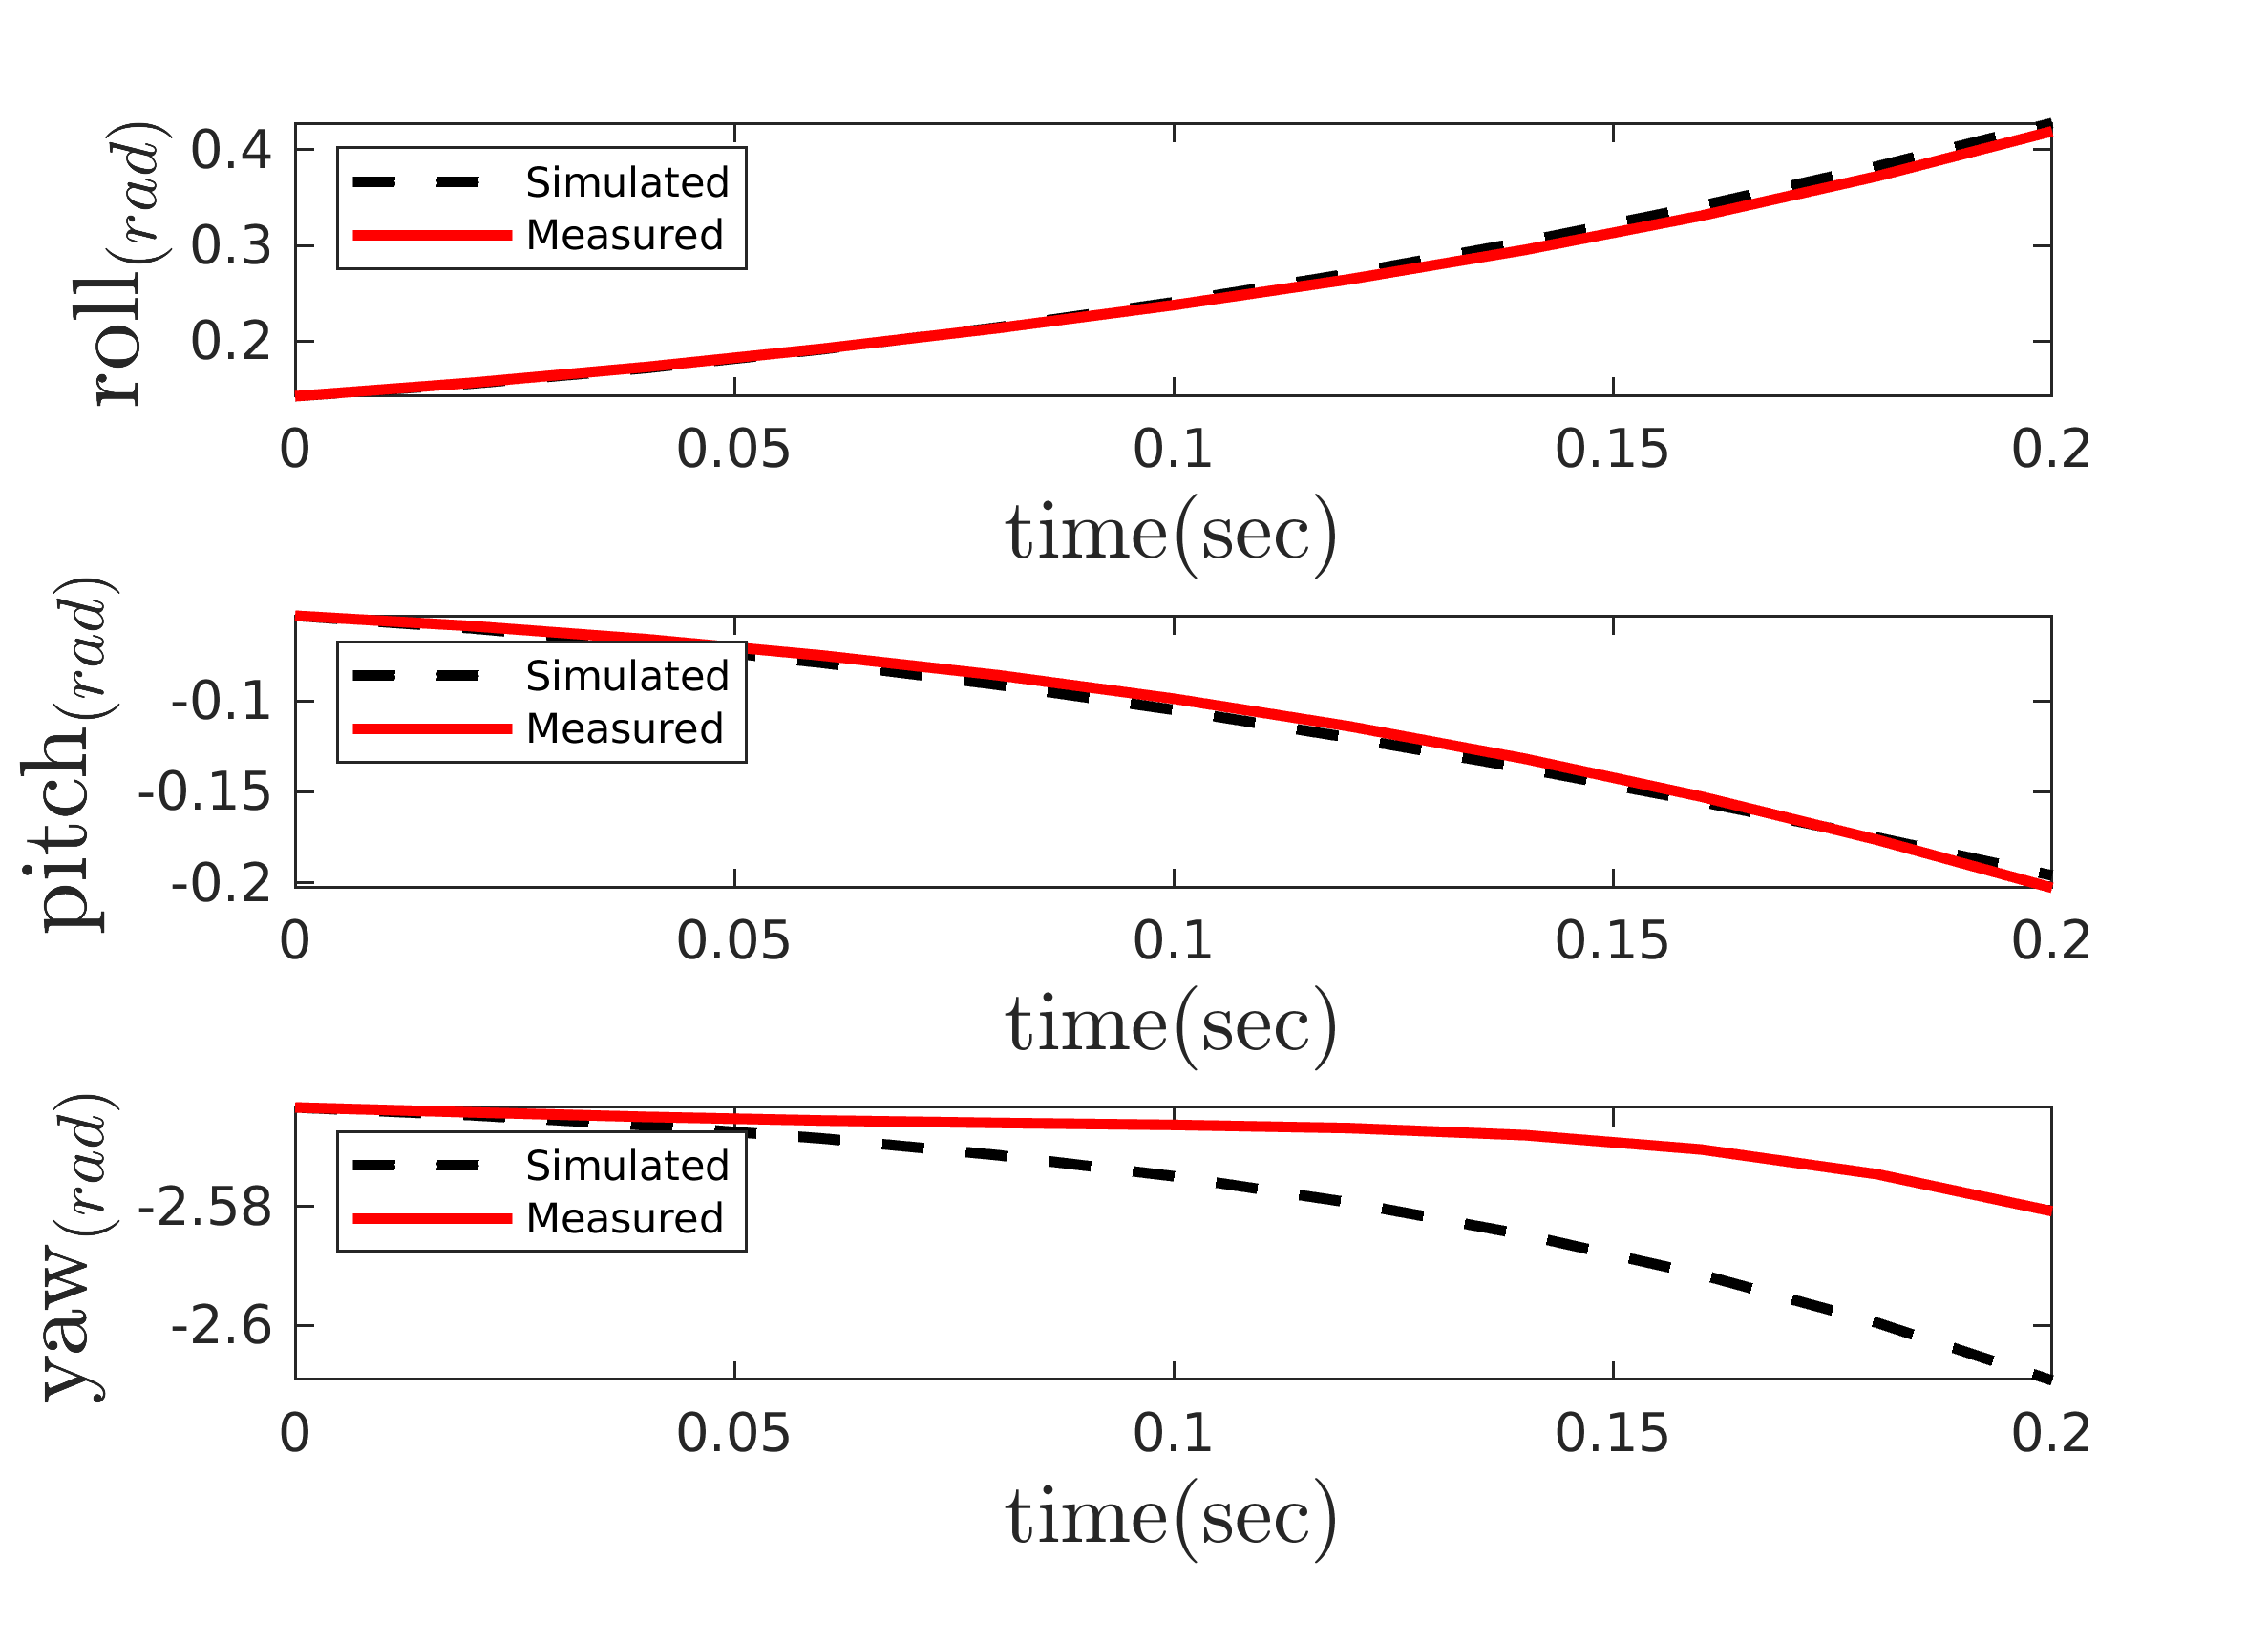
\includegraphics[width=12cm]{../../Figures/RCP/roll_pitch_yaw_parameter_estimation/RCP_roll_pitch_yaw_S5.png}
	\centering
	\caption{مقايسه وضعیت استند در  آزمايش چهارم و شبیه‌سازی، پس از تخمین پارامترهای کانال رول-پیچ-یاو}
	\label{ roll_pitch_yaw_ps4}
\end{figure}
\begin{figure}[H]
	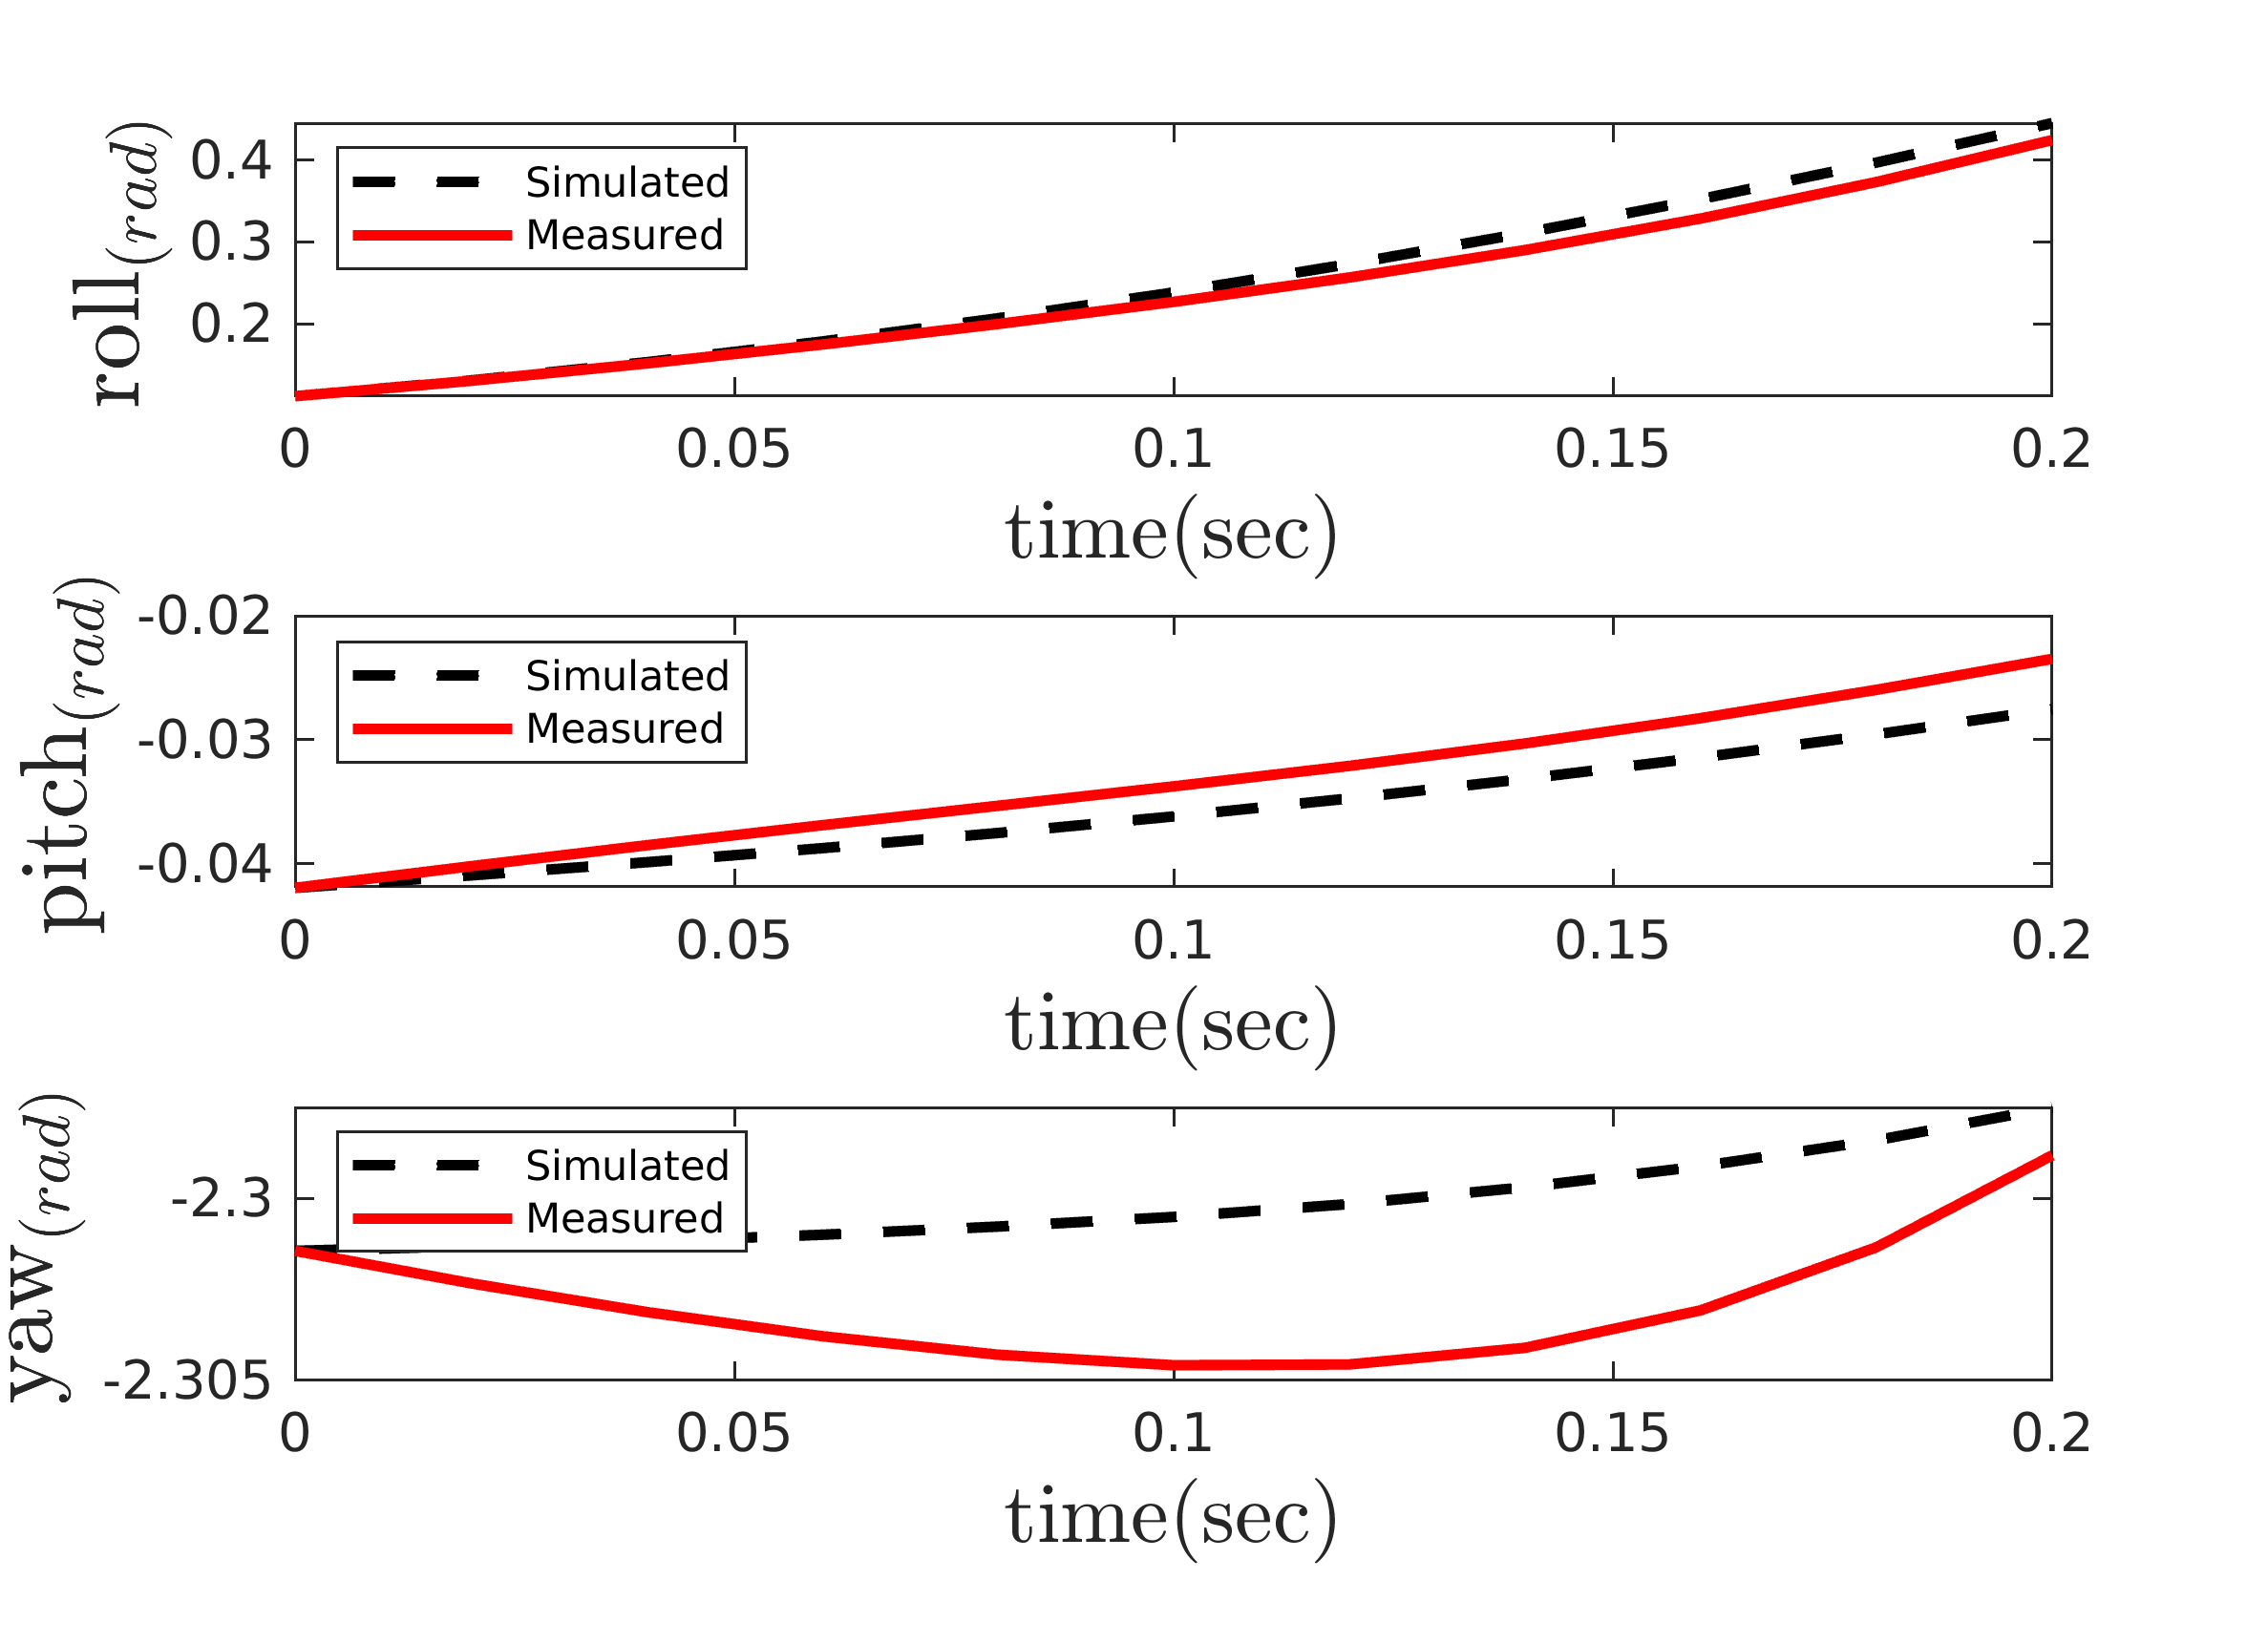
\includegraphics[width=12cm]{../../Figures/RCP/roll_pitch_yaw_parameter_estimation/RCP_roll_pitch_yaw_S6.png}
	\centering
	\caption{مقايسه وضعیت استند در  آزمايش پنجم و شبیه‌سازی، پس از تخمین پارامترهای کانال رول-پیچ-یاو}
	\label{ roll_pitch_yaw_ps5}
\end{figure}
\begin{figure}[H]
	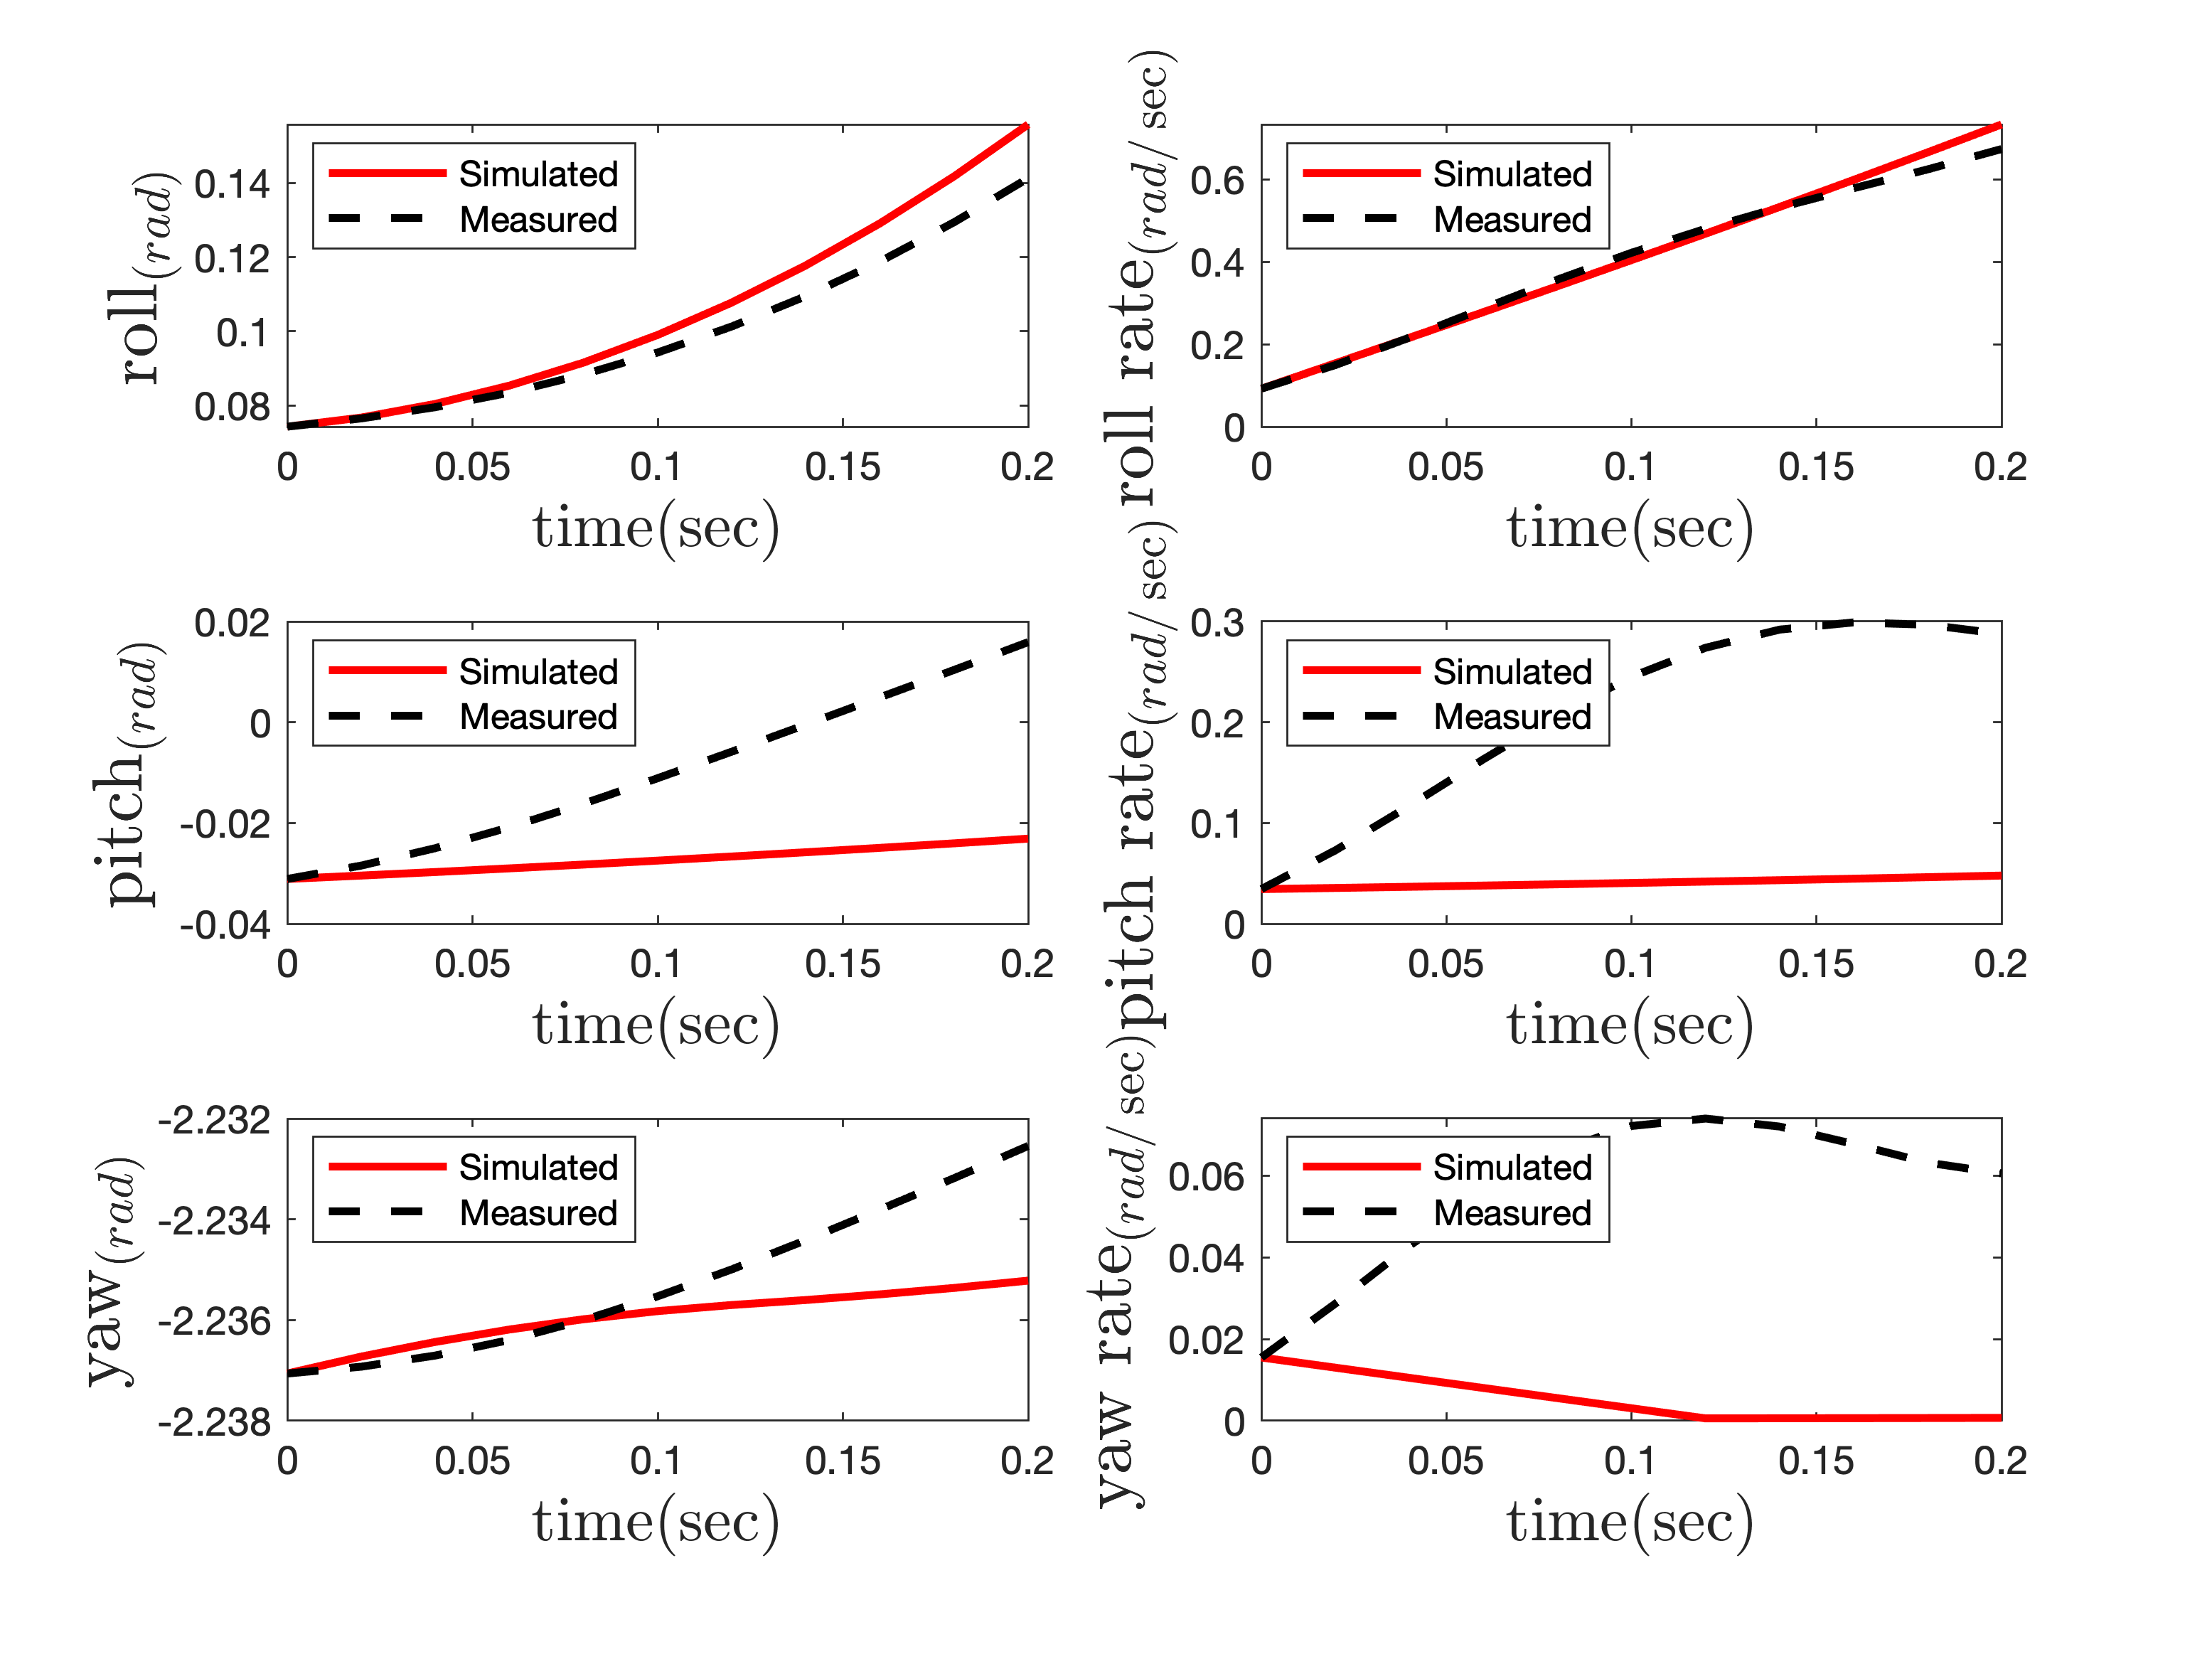
\includegraphics[width=12cm]{../../Figures/RCP/roll_pitch_yaw_parameter_estimation/RCP_roll_pitch_yaw_S7.png}
	\centering
	\caption{مقايسه وضعیت استند در  آزمايش ششم و شبیه‌سازی، پس از تخمین پارامترهای کانال رول-پیچ-یاو}
	\label{ roll_pitch_yaw_ps6}
\end{figure}
\begin{figure}[H]
	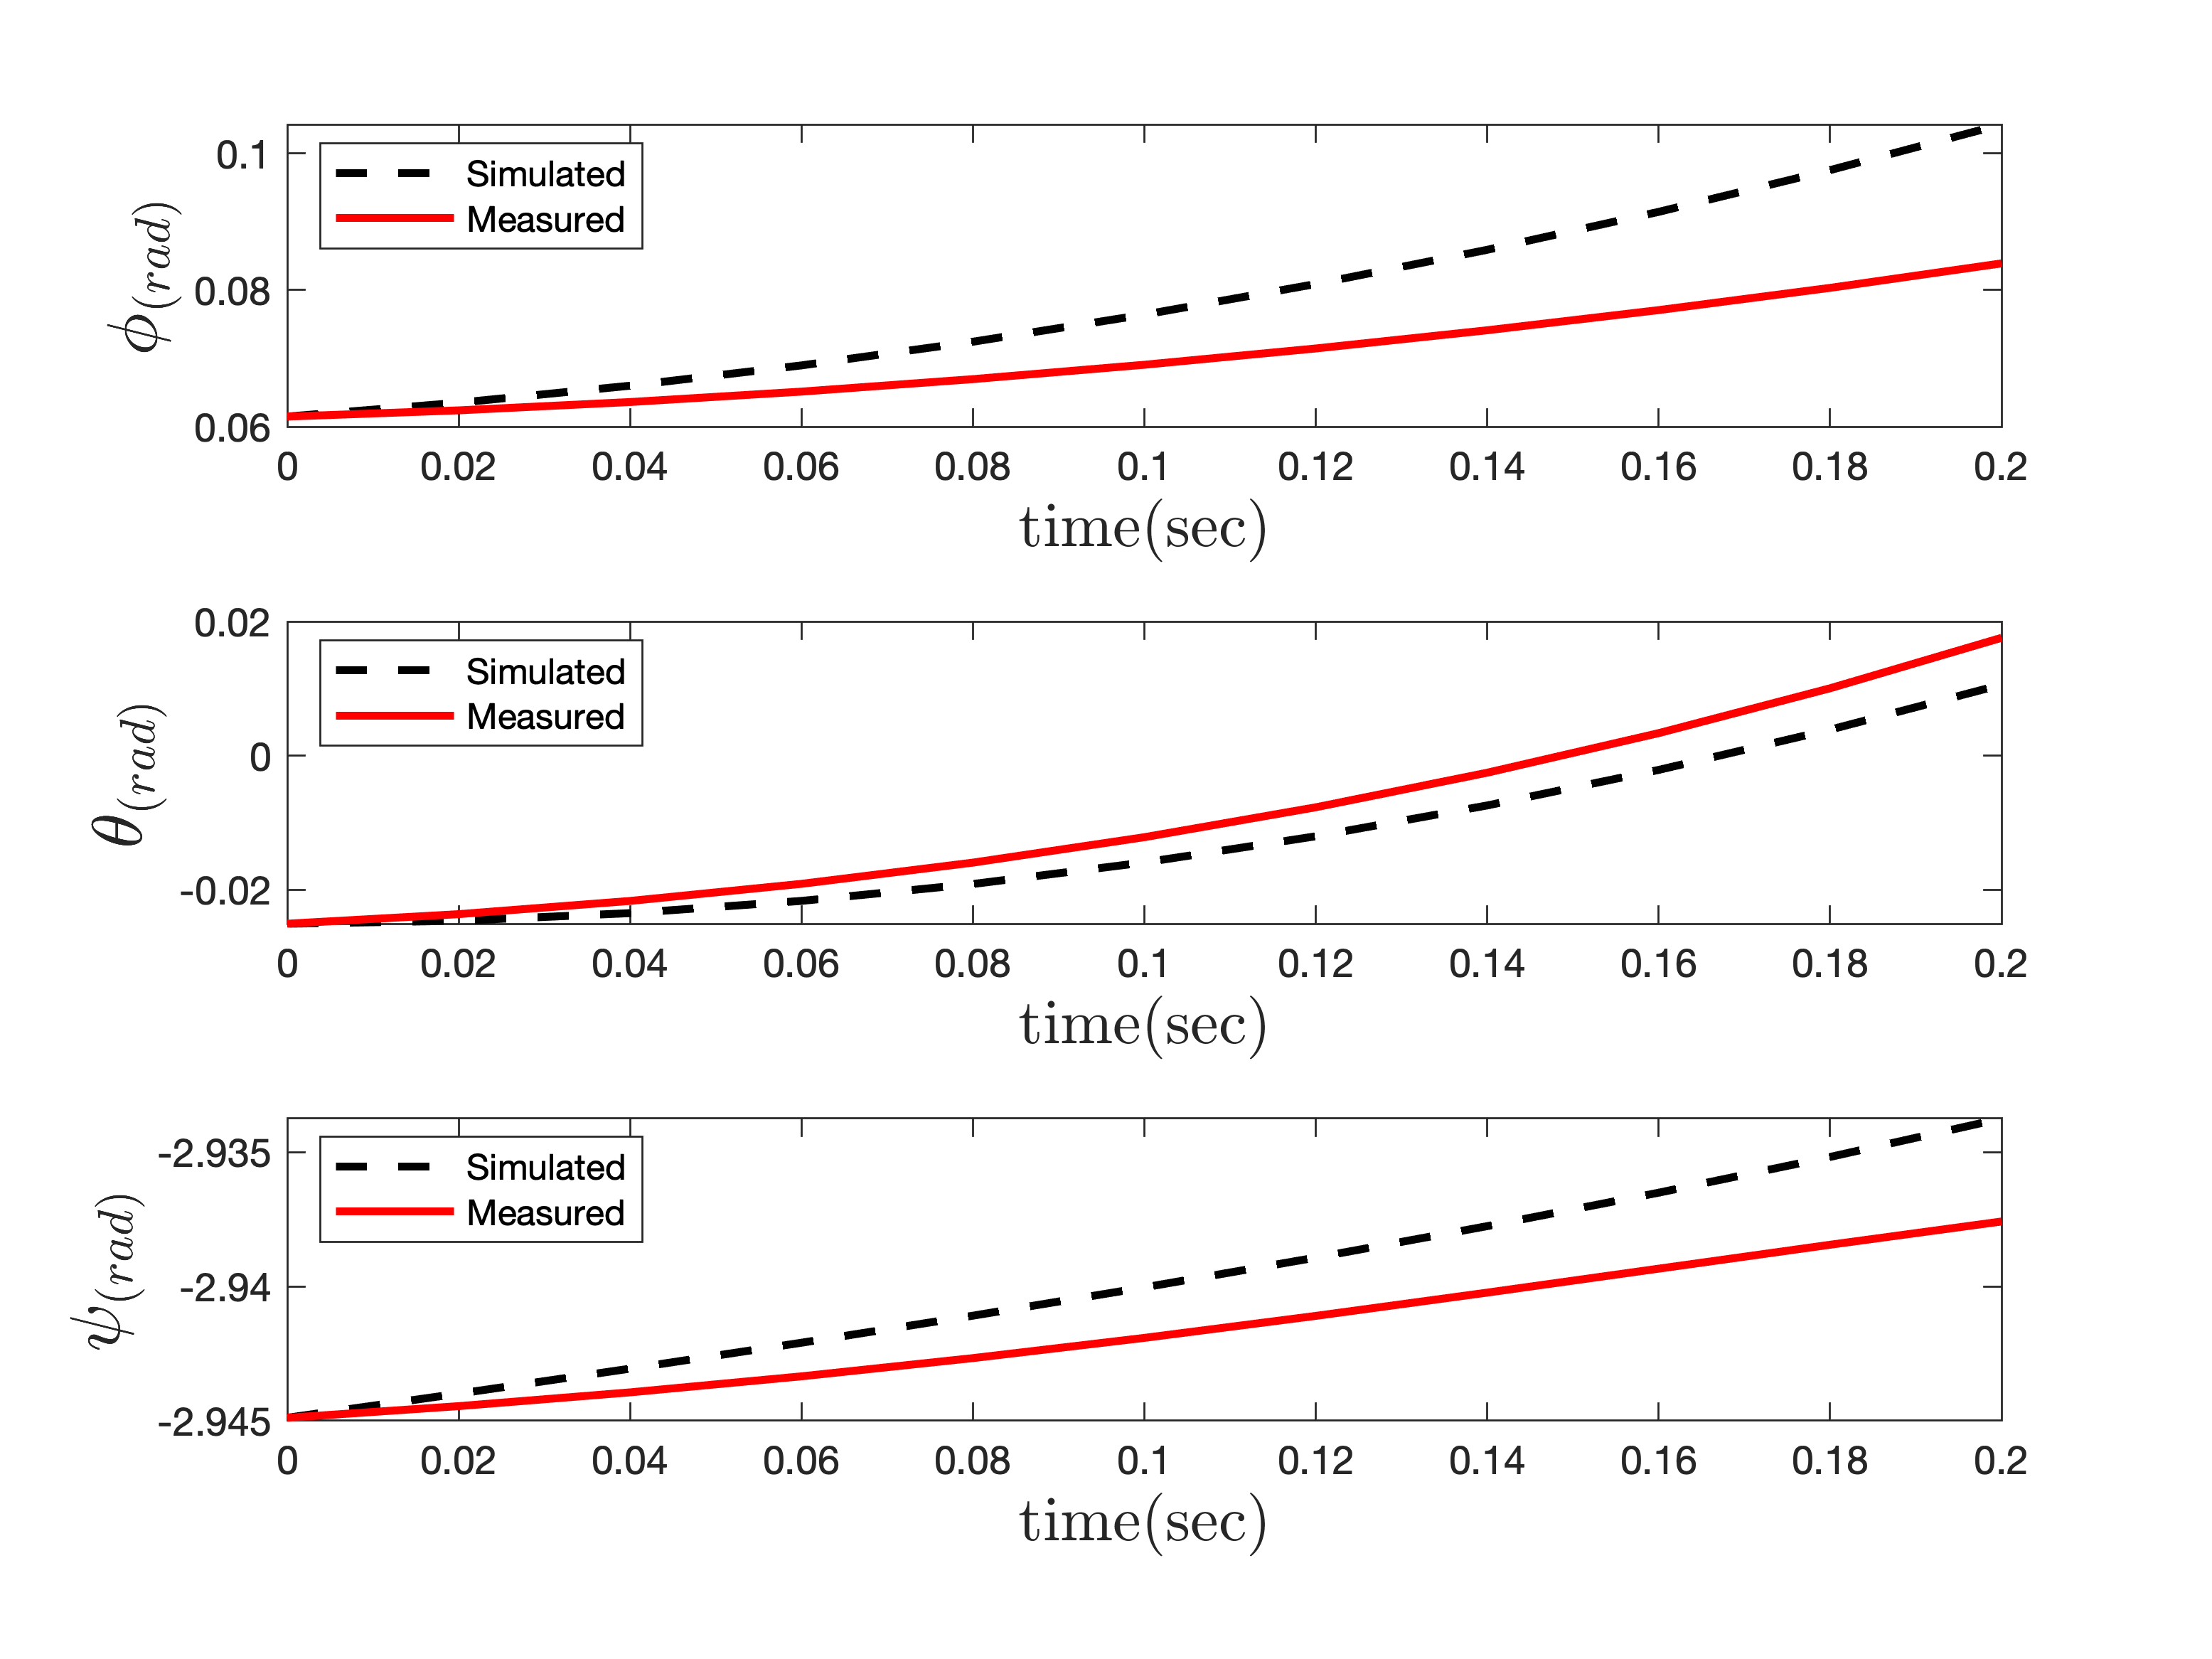
\includegraphics[width=12cm]{../../Figures/RCP/roll_pitch_yaw_parameter_estimation/RCP_roll_pitch_yaw_S8.png}
	\centering
	\caption{مقايسه وضعیت استند در  آزمايش هفتم و شبیه‌سازی، پس از تخمین پارامترهای کانال رول-پیچ-یاو}
	\label{ roll_pitch_yaw_ps7}
\end{figure}
\begin{figure}[H]
	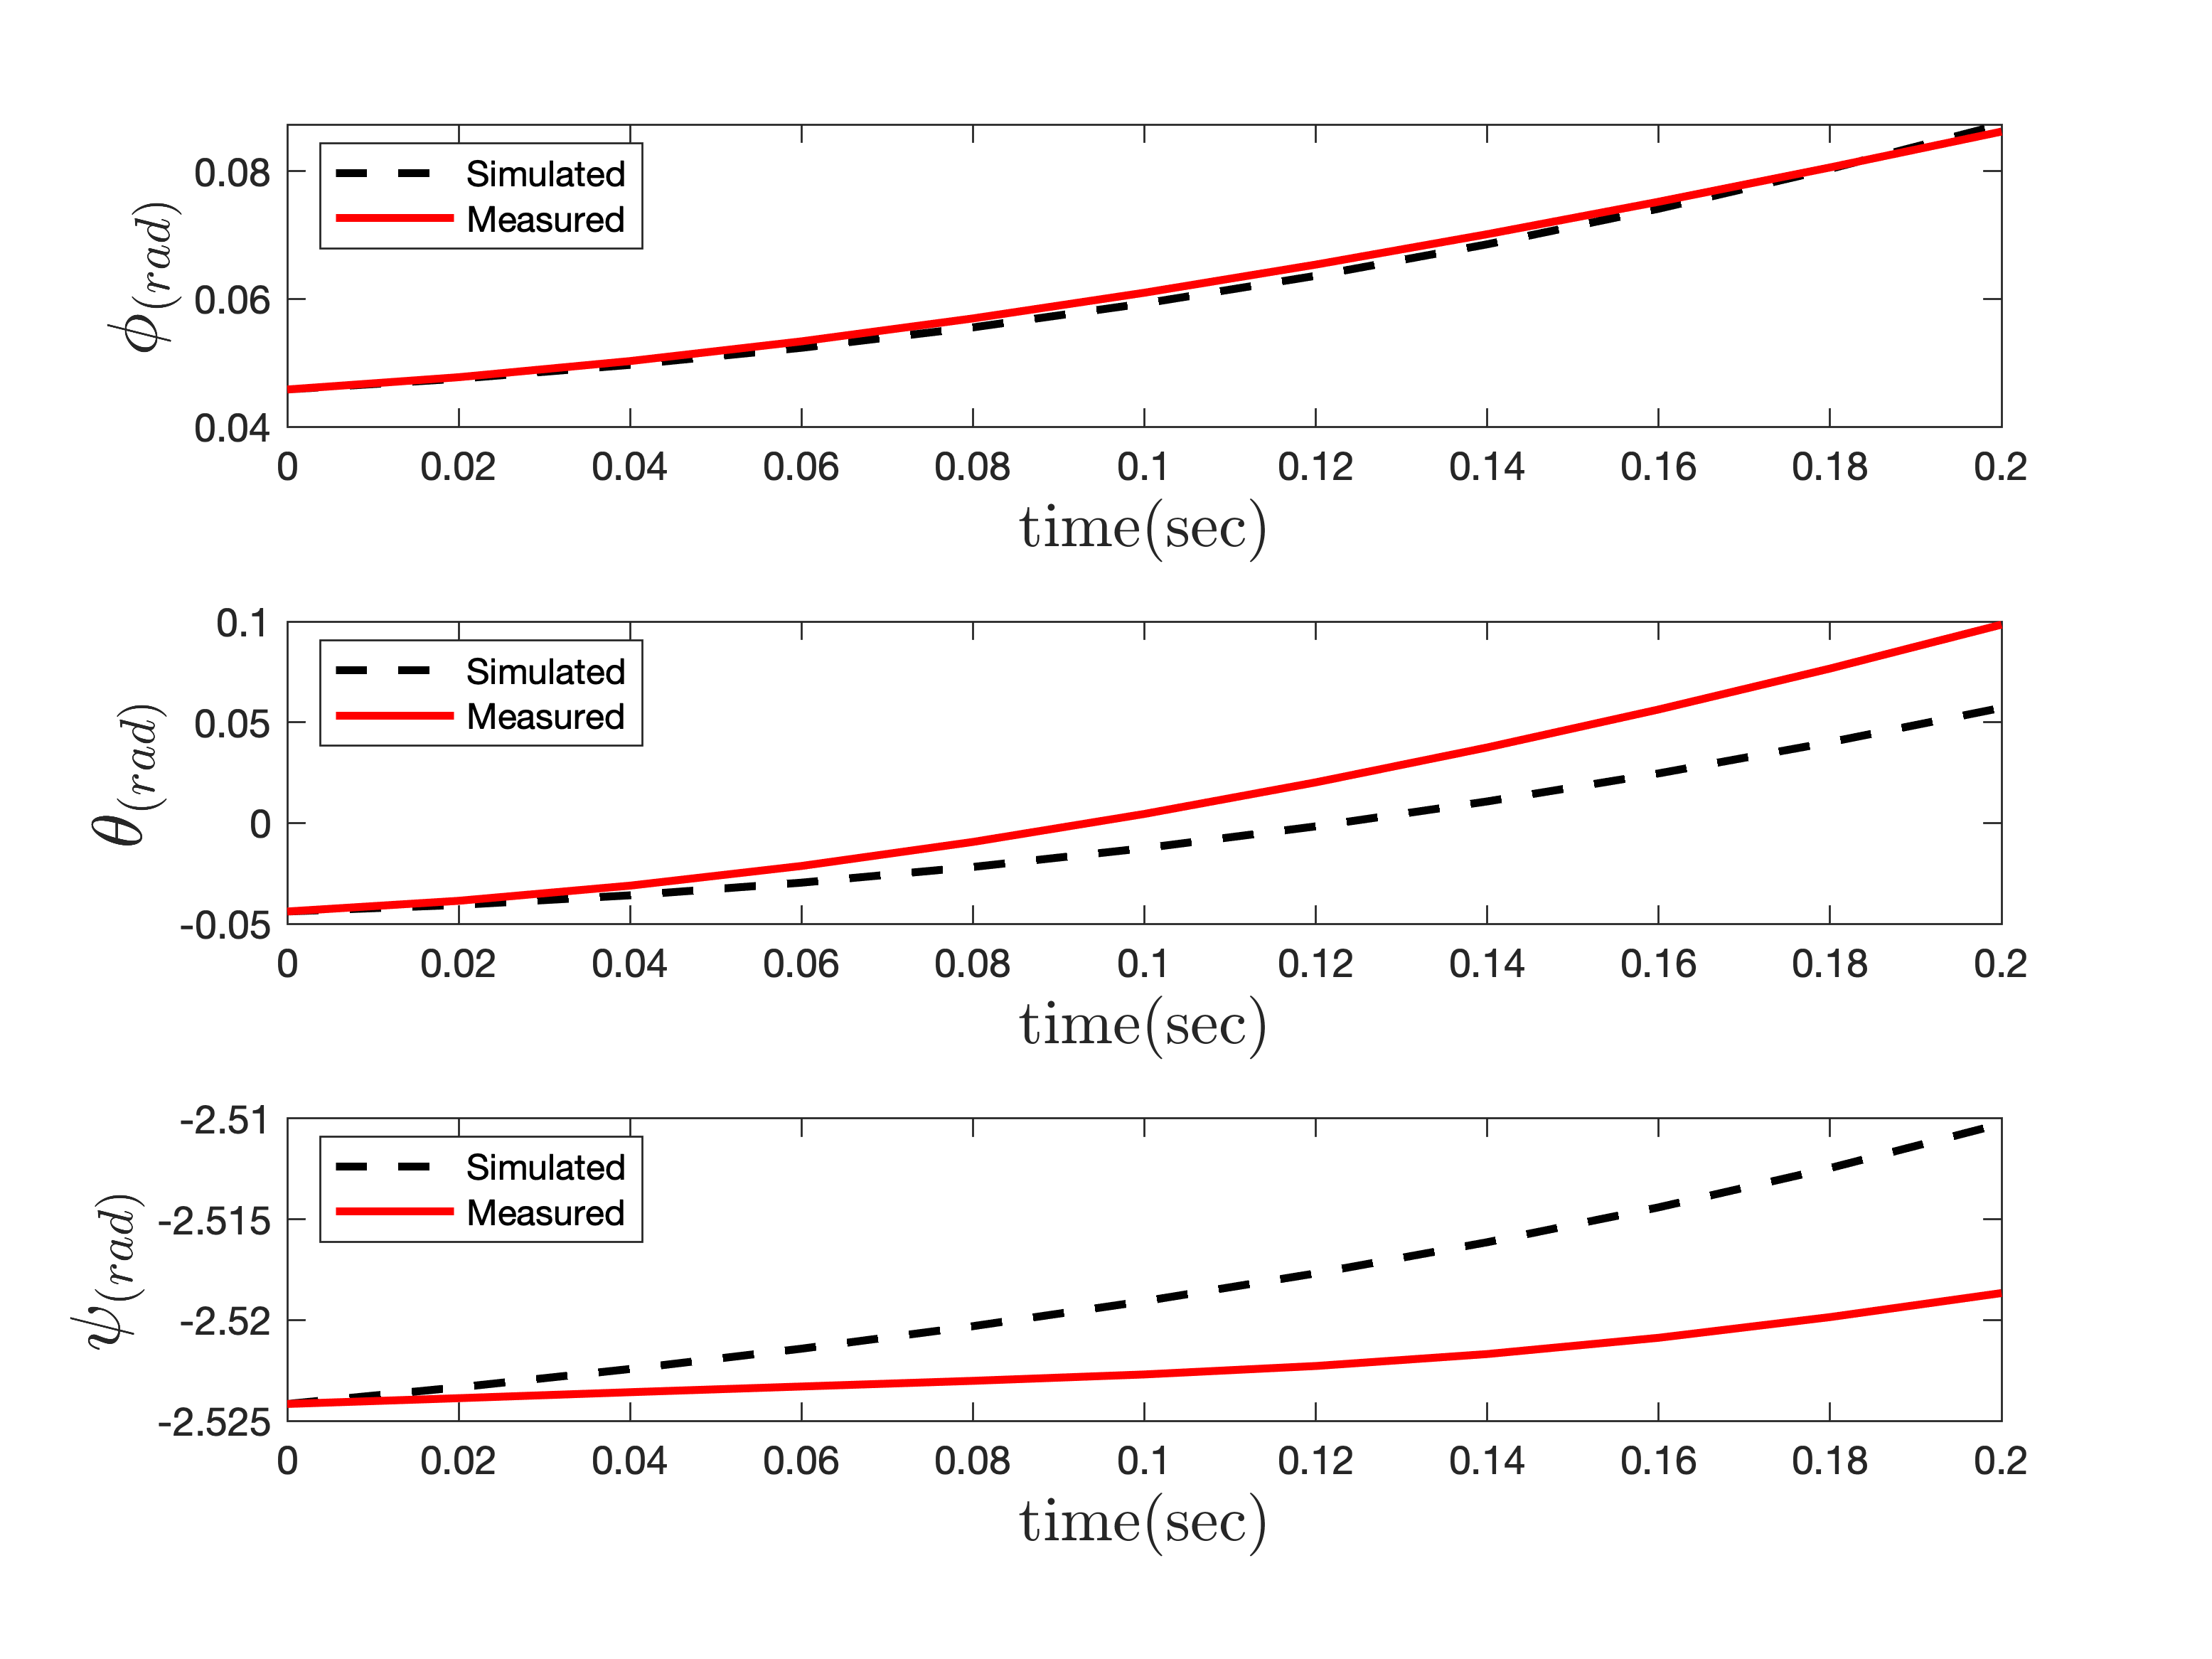
\includegraphics[width=12cm]{../../Figures/RCP/roll_pitch_yaw_parameter_estimation/RCP_roll_pitch_yaw_S9.png}
	\centering
	\caption{مقايسه وضعیت استند در  آزمايش هشتم و شبیه‌سازی، پس از تخمین پارامترهای کانال رول-پیچ-یاو}
	\label{ roll_pitch_yaw_ps8}
\end{figure}
\begin{figure}[H]
	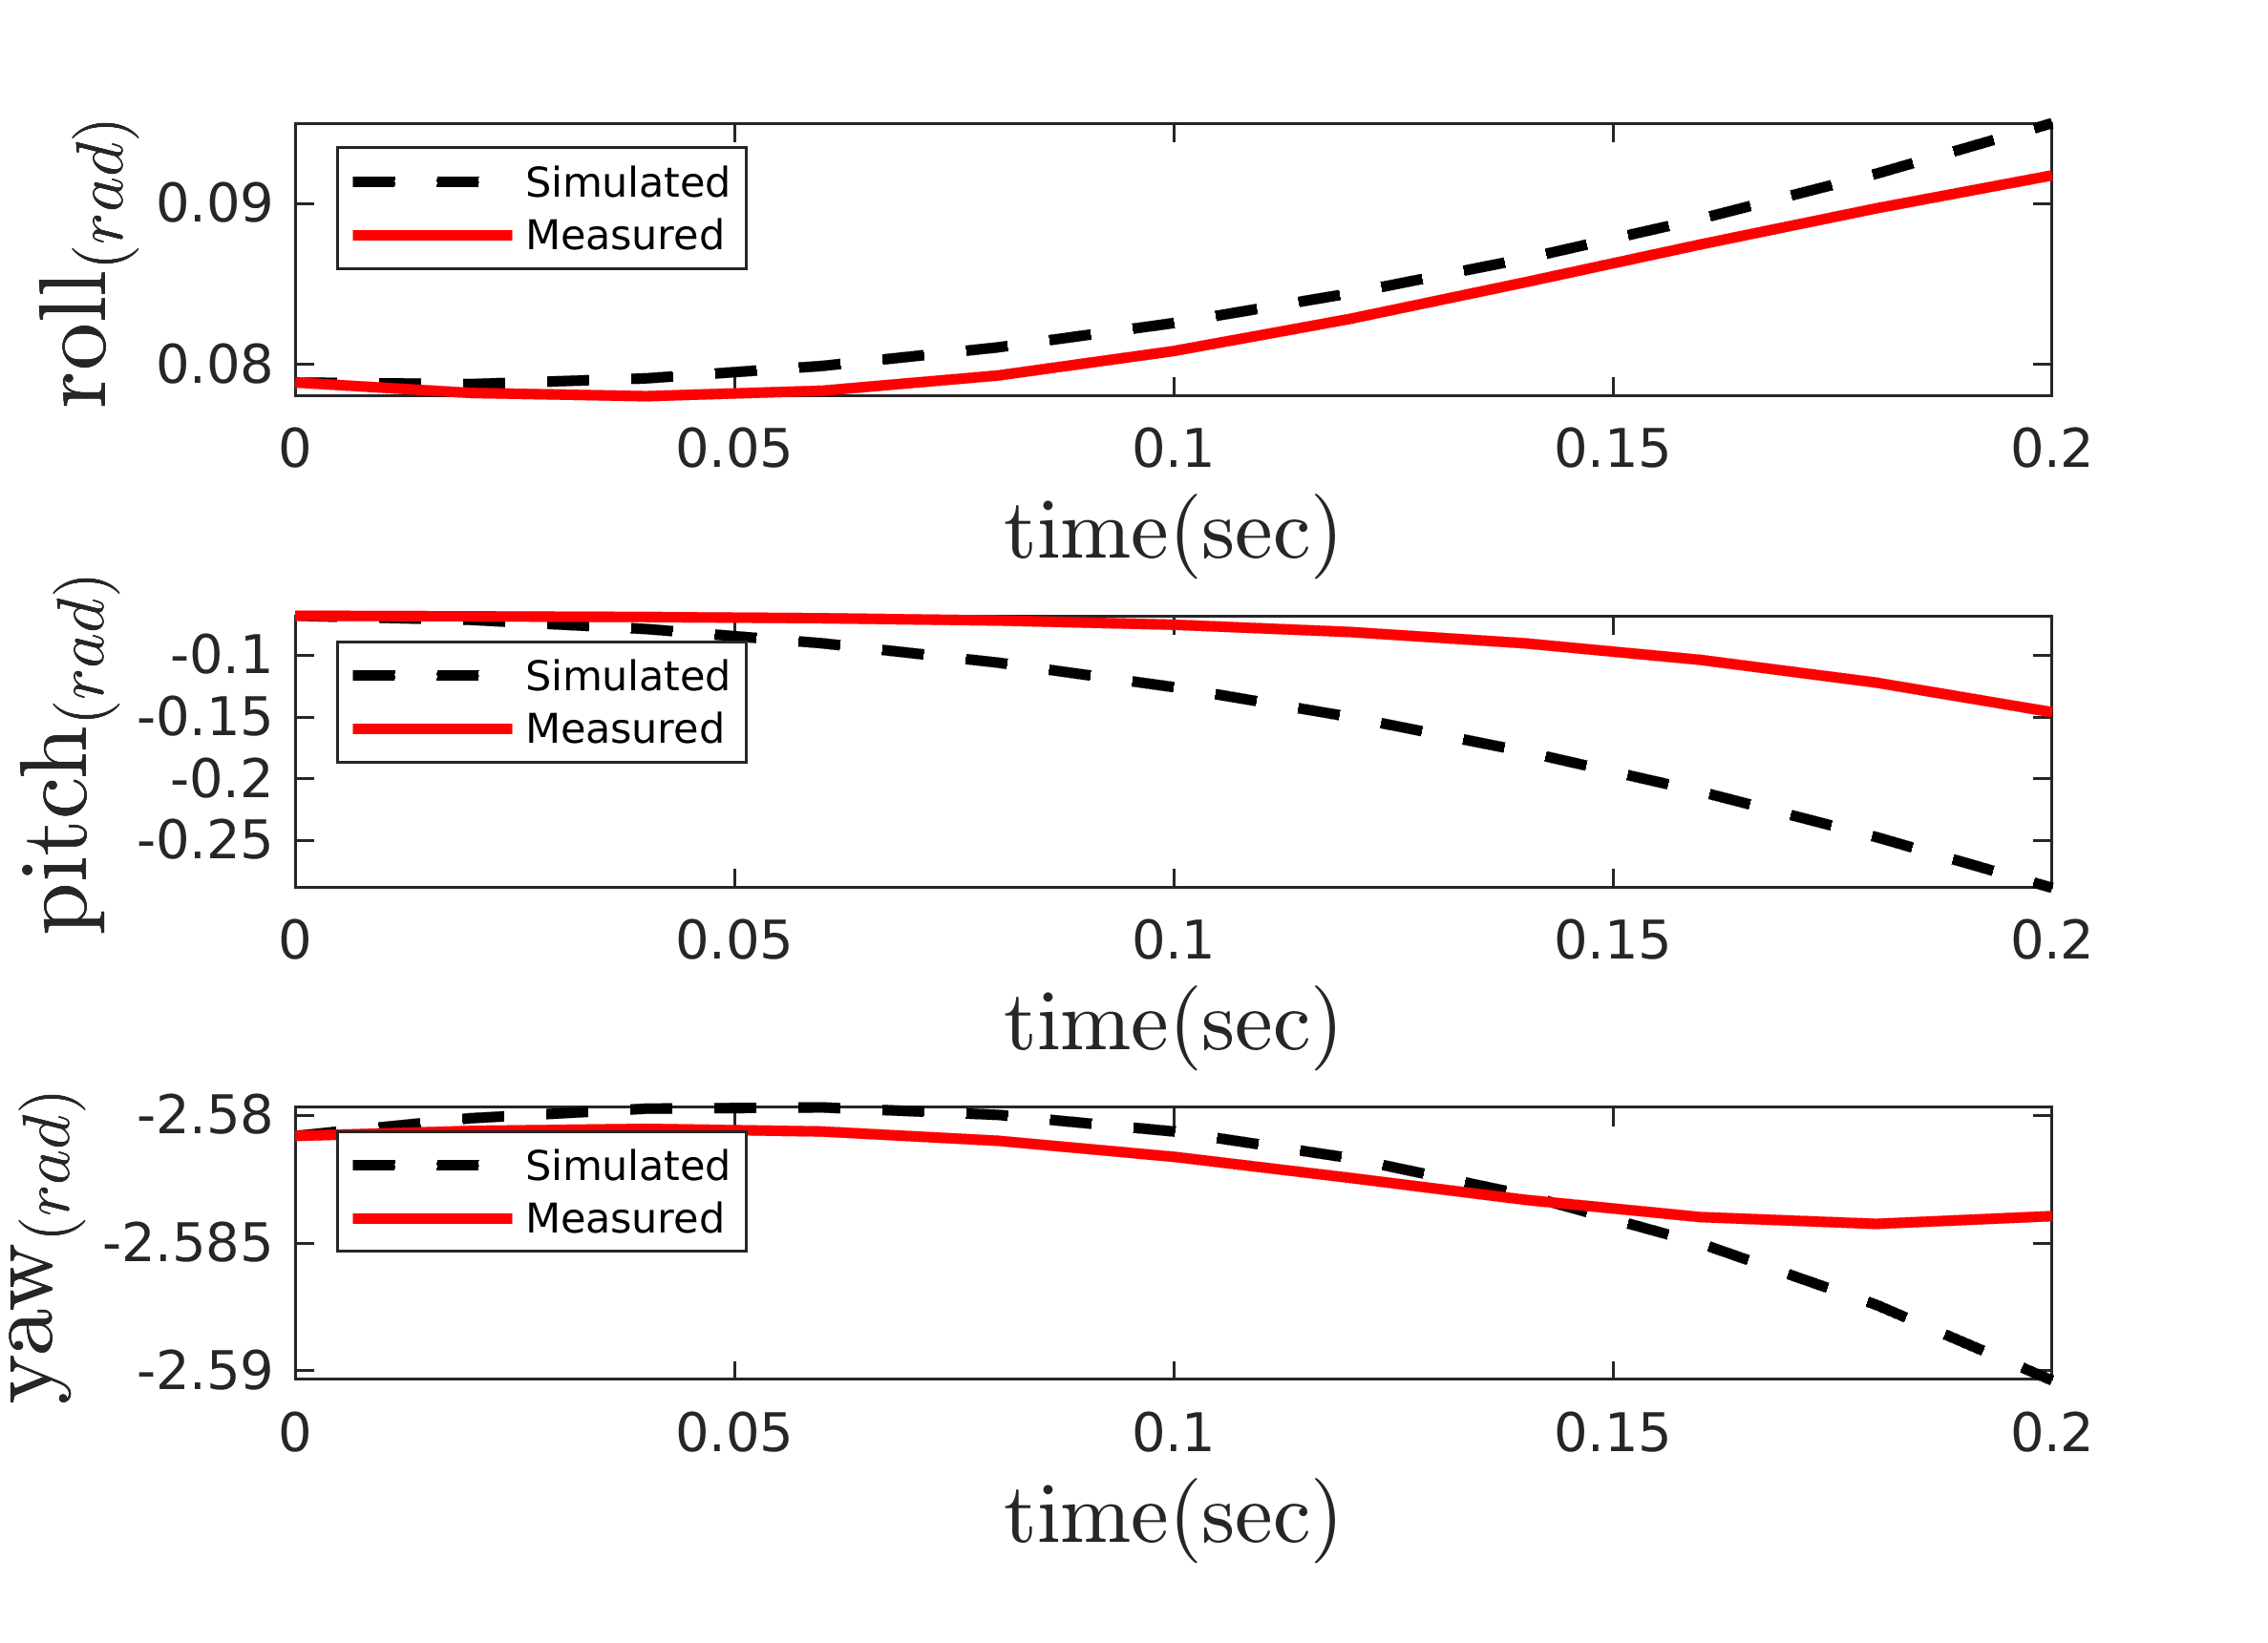
\includegraphics[width=12cm]{../../Figures/RCP/roll_pitch_yaw_parameter_estimation/RCP_roll_pitch_yaw_S10.png}
	\centering
	\caption{مقايسه وضعیت استند در  آزمايش نهم و شبیه‌سازی، پس از تخمین پارامترهای کانال رول-پیچ-یاو}
	\label{ roll_pitch_yaw_ps9}
\end{figure}
